\documentclass[11pt,a4paper]{article}
\usepackage[T1]{fontenc}
\usepackage[utf8]{inputenc}
\usepackage[top=2.2cm, bottom=2.2cm, left=2.5cm, right=2.5cm]{geometry}
\usepackage{graphicx}
\usepackage{enumitem}
\usepackage{fancyvrb}
\usepackage{array}

\setlength{\parindent}{0pt}
\setlength{\parskip}{0.5em}
\linespread{1.08}

\setlist[itemize]{topsep=2pt, itemsep=3pt, parsep=0pt, leftmargin=1.5em}

\fvset{
    fontsize=\footnotesize,
    frame=single,
    framesep=5pt,
    samepage=false,
    xleftmargin=2pt,
    xrightmargin=2pt
}

\title{\textbf{Report.10.DB.Design.Magazine}\\[0.3em]\large Database Design Report -- Magazine Database}
\author{Tran Bao Ngoc \\ Student ID: 2640118}
\date{Information Systems (MI1.02a) \\ Labwork 05 -- Database design (exercise 1: magazine)}

\begin{document}
\maketitle

\section{The problem}
I need a database for the magazines I buy regularly. For every magazine I keep the title, the ISSN (the code that identifies the publication), the number and the year. I also keep the articles: title, starting page and ending page. No two articles have the same title. An article can have several authors, and for each author I store the name, e-mail address and affiliation, plus a number telling the order of the authors on that article.

\section{How I made the structure}

\subsection{Conceptual model}
Reading the text, I found three things I need to store: magazines, articles and authors.
\begin{itemize}
    \item \textbf{Magazine} has ISSN, title, number and year. The ISSN only identifies the publication, not one particular issue, so I use ISSN + number + year together as the key of an issue.
    \item \textbf{Article} has a title, a start page and an end page. Since titles are never repeated, the title is enough as its key.
    \item \textbf{Author} has a name, an e-mail and an affiliation. I chose the e-mail as the key because two authors may have the same name.
\end{itemize}

Relationships:
\begin{itemize}
    \item One magazine issue contains many articles, and each article is in exactly one issue (one-to-many).
    \item One article can have many authors and one author can write many articles (many-to-many). The order of the authors belongs to this relationship, not to the article or the author alone.
\end{itemize}

\subsection{Logical model}
\begin{itemize}
    \item \texttt{Magazine(\underline{ISSN, Number, Year}, Title)} \\
    Primary key: \texttt{(ISSN, Number, Year)}
    \item \texttt{Article(\underline{ArticleTitle}, StartPage, EndPage, ISSN, Number, Year)} \\
    Primary key: \texttt{ArticleTitle}; Foreign key: \texttt{(ISSN, Number, Year)} $\rightarrow$ \texttt{Magazine}
    \item \texttt{Author(\underline{Email}, AuthorName, Affiliation)} \\
    Primary key: \texttt{Email}
    \item \texttt{Article\_author(\underline{ArticleTitle, Email}, AuthorOrder)} \\
    Primary key: \texttt{(ArticleTitle, Email)}; Foreign keys: \texttt{ArticleTitle} $\rightarrow$ \texttt{Article}, \texttt{Email} $\rightarrow$ \texttt{Author}
\end{itemize}

The many-to-many relationship becomes the table \texttt{Article\_author}, and \texttt{AuthorOrder} is stored there.

About normal forms: every column holds a single value, so the tables are in 1NF. Article, Author and Article\_author have no partial or transitive dependencies. The one weak point is Magazine: the title depends only on the ISSN, so it is repeated for every issue of the same magazine. I left it like this to keep the model close to the description of the exercise. Splitting the title into its own table would fix it.

\subsection{Physical model}
The ER diagram is in \texttt{Labwork-05a.png}. I used VARCHAR for names, titles and e-mails, and INT for pages, numbers and years. All foreign keys use \texttt{ON UPDATE CASCADE} and \texttt{ON DELETE CASCADE}, so deleting an issue also deletes its articles.

\IfFileExists{Labwork-05a.png}{%
    \begin{center}
        \vspace{0.3em}
        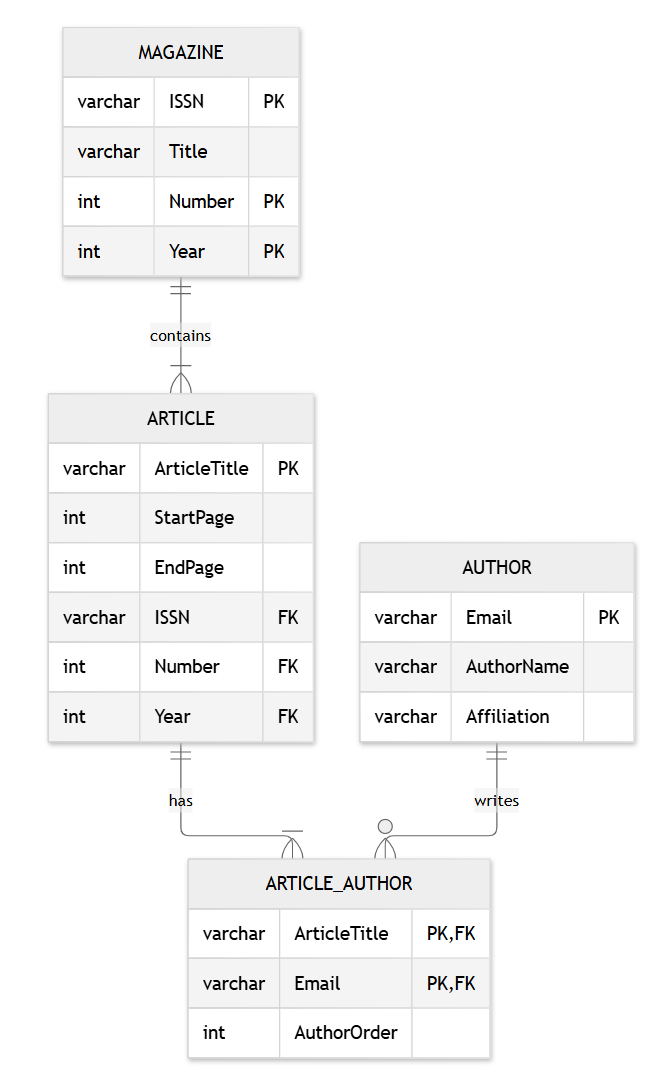
\includegraphics[width=0.85\textwidth, height=0.35\textheight, keepaspectratio]{Labwork-05a.png}
        \vspace{0.3em}
    \end{center}
}{}

\newpage
\section{SQL commands to create the database}
\begin{Verbatim}
DROP DATABASE IF EXISTS magazine_db;
CREATE DATABASE magazine_db;
USE magazine_db;

-- 1. Table: Magazine
CREATE TABLE MAGAZINE (
    ISSN VARCHAR(20) NOT NULL,
    Title VARCHAR(255) NOT NULL,
    Number INT NOT NULL,
    Year INT NOT NULL,
    PRIMARY KEY (ISSN, Number, Year)
);

-- 2. Table: Article
CREATE TABLE ARTICLE (
    ArticleTitle VARCHAR(255) NOT NULL,
    StartPage INT NOT NULL,
    EndPage INT NOT NULL,
    ISSN VARCHAR(20) NOT NULL,
    Number INT NOT NULL,
    Year INT NOT NULL,
    PRIMARY KEY (ArticleTitle),
    FOREIGN KEY (ISSN, Number, Year) REFERENCES MAGAZINE(ISSN, Number, Year)
        ON UPDATE CASCADE ON DELETE CASCADE
);

-- 3. Table: Author
CREATE TABLE AUTHOR (
    Email VARCHAR(255) NOT NULL,
    AuthorName VARCHAR(255) NOT NULL,
    Affiliation VARCHAR(255),
    PRIMARY KEY (Email)
);

-- 4. Table: Article_author
CREATE TABLE ARTICLE_AUTHOR (
    ArticleTitle VARCHAR(255) NOT NULL,
    Email VARCHAR(255) NOT NULL,
    AuthorOrder INT NOT NULL,
    PRIMARY KEY (ArticleTitle, Email),
    FOREIGN KEY (ArticleTitle) REFERENCES ARTICLE(ArticleTitle)
        ON UPDATE CASCADE ON DELETE CASCADE,
    FOREIGN KEY (Email) REFERENCES AUTHOR(Email)
        ON UPDATE CASCADE ON DELETE CASCADE
);
\end{Verbatim}

\newpage
\section{DESCRIBE commands and their outputs}
\begin{Verbatim}
-- DESCRIBE MAGAZINE;
+--------+--------------+------+-----+---------+-------+
| Field  | Type         | Null | Key | Default | Extra |
+--------+--------------+------+-----+---------+-------+
| ISSN   | varchar(20)  | NO   | PRI | NULL    |       |
| Title  | varchar(255) | NO   |     | NULL    |       |
| Number | int          | NO   | PRI | NULL    |       |
| Year   | int          | NO   | PRI | NULL    |       |
+--------+--------------+------+-----+---------+-------+

-- DESCRIBE ARTICLE;
+--------------+--------------+------+-----+---------+-------+
| Field        | Type         | Null | Key | Default | Extra |
+--------------+--------------+------+-----+---------+-------+
| ArticleTitle | varchar(255) | NO   | PRI | NULL    |       |
| StartPage    | int          | NO   |     | NULL    |       |
| EndPage      | int          | NO   |     | NULL    |       |
| ISSN         | varchar(20)  | NO   | MUL | NULL    |       |
| Number       | int          | NO   |     | NULL    |       |
| Year         | int          | NO   |     | NULL    |       |
+--------------+--------------+------+-----+---------+-------+

-- DESCRIBE AUTHOR;
+-------------+--------------+------+-----+---------+-------+
| Field       | Type         | Null | Key | Default | Extra |
+-------------+--------------+------+-----+---------+-------+
| Email       | varchar(255) | NO   | PRI | NULL    |       |
| AuthorName  | varchar(255) | NO   |     | NULL    |       |
| Affiliation | varchar(255) | YES  |     | NULL    |       |
+-------------+--------------+------+-----+---------+-------+

-- DESCRIBE ARTICLE_AUTHOR;
+--------------+--------------+------+-----+---------+-------+
| Field        | Type         | Null | Key | Default | Extra |
+--------------+--------------+------+-----+---------+-------+
| ArticleTitle | varchar(255) | NO   | PRI | NULL    |       |
| Email        | varchar(255) | NO   | PRI | NULL    |       |
| AuthorOrder  | int          | NO   |     | NULL    |       |
+--------------+--------------+------+-----+---------+-------+
\end{Verbatim}

\end{document}